% ==============================================================================
\subsection{Small Perturbation Model}
We get the linearised model using small perturbtation and neglecting the gain variation $(\delta v)$:
\begin{align*}
    J \delta \dot \omega + b_m \delta \omega + 2 C_D \omega_0 \delta \omega  &= \delta u_\omega \lr{V_{in} b_m + 2V_{in}^2 C_D u_{\omega_0}}\\
    J \delta \dot \omega + (b_m + 2 C_D \omega_0) \delta \omega  &= \delta u_\omega \lr{V_{in} b_m + 2V_{in}^2 C_D u_{\omega_0}}\\
    \text{Laplace Transform:} \qquad \qquad &\\
     \lr{Js + (b_m + 2 C_D \omega_0)} \delta \omega  &= \delta u_\omega \lr{V_{in} b_m + 2V_{in}^2 C_D u_{\omega_0}}
\end{align*}
Thus we have the trannsfer function model:
\begin{align*}
    \frac{\delta \omega(s)}{\delta u_\omega (s)} &= \frac{V_{in} b_m + 2V_{in}^2 C_D u_{\omega_0}}{Js + (b_m + 2 C_D \omega_0)}
\end{align*}
Also, we have the following relationship between the nominal input and outputs from the input-definition:
\begin{align*}
    \omega_0 &= V_{in} u_{\omega_0}\\
    \implies \frac{\delta \omega(s)}{\delta u_\omega (s)} &= \frac{V_{in} \lr{b_m + 2C_D V_{in} u_{\omega_0}}}{Js + (b_m + 2 C_D \omega_0)}
    = \frac{V_{in} \lr{b_m + 2C_D \omega_0}}{Js + (b_m + 2 C_D \omega_0)}\\
    &= \frac{V_{in}}{ \lr{\frac{J}{b_m + 2 C_D \omega_0}} s + 1} \quad \lr{= \frac{K_m}{\tau_m s + 1}}\\
    \implies K_m &= V_{in}\\
    \tau_m &= \frac{J}{b_m + 2 C_D \omega_0}\\
    \implies \omega_m &= \frac{1}{J}\lr{b_m + 2 C_D \omega_0}
\end{align*}

Thus time-constant decreases with the nominal rpm and the static gain is purely a funciton on the battery voltage.

This information will be used for establishing the validity of identified model. Sum-of-Sinusoids input is used around a nominal input for generating the frequency response of the system to identify the model.

In case of using $u_p$ as input:
\begin{align*}
    u_\omega &= a u_p + b\\
    \implies \delta u_\omega &= a \delta u_p\\
    \implies \frac{\delta \omega(s)}{\delta u_p(s)} &= \lr{\frac{1}{a}}\frac{K_m}{\tau_m s + 1}
\end{align*}

Thus this results in variation of the static gain alone.


\subsubsection{Linearized Model Parameter Estimation}
The response of the system to Sum-of-Sinusoids signal at $250 \, Hz$ and $50 \mu s$ (PWM) amplitude containing $299$ frequencies in the range $[0.01, 30]\,Hz$ is used for first-order model parameter identification. The nominal inputs and the corresponding $rpm$ is tabulated in Table~\ref{tab::nom_in}. The identified models are validated against the response of a chirp signal with the same frequency range and sampling frequency. The validation results are plotted in Section~\ref{sec::small_perturb_valid}.

The estimates static-gain and cut-off frequencies are plotted with nominal inputs. The corresopnding parameters relating them to the nominal inputs are estimated using least-squares method.

The $V_{in}$ and $K$ plot demonstrates the validity of their relationship when the $V_{in}$ variation is inclued, i.e.,
\begin{align*}
    K &= V_{in} (1 + \delta v)
\end{align*}

The variation of cut-off frequency with nominal rpm gives the esitmates of propeller moment of inertia and the damping as follows:
\begin{align*}
    J &= 3.2238 \times 10^{-6} \, Kg .m^2\\
    b_m &= 0
\end{align*}

\begin{figure}[H]
    \centering
    \begin{minipage}{0.49\textwidth}
        \begin{figure}[H]
            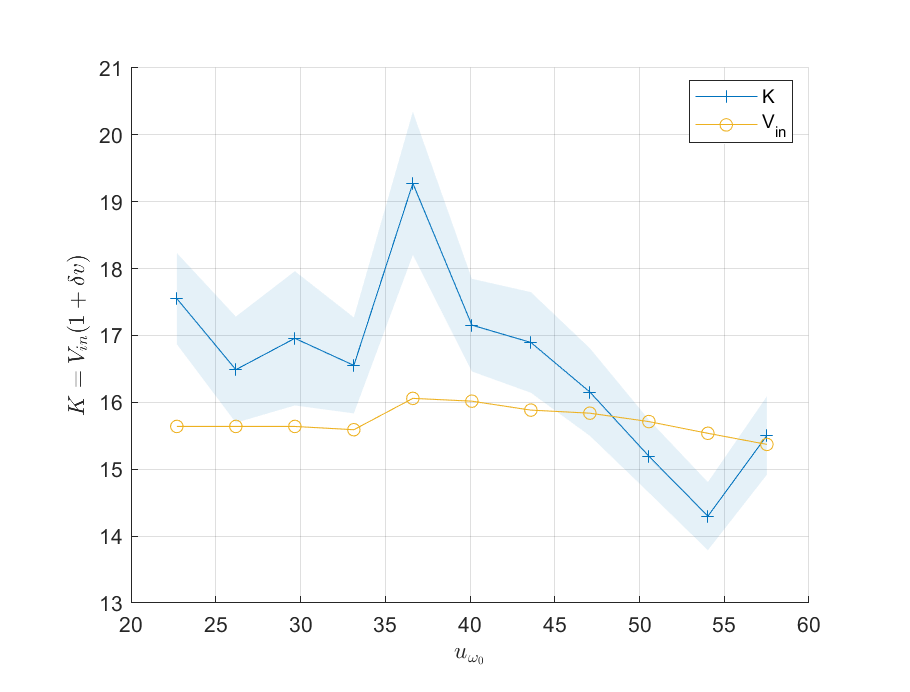
\includegraphics[width = \textwidth]{./figs/small_perturbation/K-Vin.eps}
            \caption{Static gain and Voltage input}
        \end{figure}
    \end{minipage}
    \begin{minipage}{0.49\textwidth}
        \begin{figure}[H]
            \includegraphics[width = \textwidth]{./figs/small_perturbation/omega_fit.eps}
            \caption{Cut-off frequency}
        \end{figure}
    \end{minipage}
\end{figure}



\subsubsection{Validation using the response of the full non-linear model}
We have the model parameters identified:
\begin{table}[H]
    \centering
    \begin{tabular}{c l l}
        \hline \hline
        Parameter & Value & \\ \hline \hline
        $C_T$ & $7.2581 \times 10^{-06}$ & $N/(rad/s)^2$  \\
        $C_D$ & $3.6088 \times 10^{-08}$ & $N.m/(rad/s)^2$ \\
        $b_m$ & $0.0$                    & $N.m/(rad/s)$\\
        $M_f$ & $1.3135 \times 10^{-3}$  & $N.m$\\
        $J$   & $3.2238 \times 10^{-6}$  & $Kg .m^2$ \\\hline \hline
    \end{tabular}
    \caption{Summary of parameter estimates from staic and small-perturbation experiments}
\end{table}

Assuming $\delta v = 0$ we have the non-linear model of the system eqn~\ref{eqn::nl_model}:
\begin{align*}
    J \dot \omega + b_m \omega + C_D \omega^2 = V_{in} b_m u_\omega + V_{in}^2 C_D u_\omega^2
\end{align*}
The above model is simulated with the identified parameters using a square wave and chirp input whose amplitude covers the full operating range. The results of the simulation are then compared with the experimental data.
\begin{figure}[H]
    \begin{minipage}{0.49\textwidth}
        \begin{figure}[H]
            \includegraphics[width = \textwidth]{./figs/nl_valid/square_validation.eps}
            \caption*{Square Wave Input}
        \end{figure}
    \end{minipage}
    \begin{minipage}{0.49\textwidth}
        \begin{figure}[H]
            \includegraphics[width = \textwidth]{./figs/nl_valid/chirp_validation.eps}
            \caption*{Chirp Input}
        \end{figure}
    \end{minipage}
    \caption{Model Validation}
    \label{fig::model_valid}
\end{figure}

Form the Figure~\ref{fig::model_valid}, it can be concluded that the model parameters are estimated with a reasonable accuracy. The error in simulation as compared to the esperiment can be primarily attributed to theh $\delta v$ that needs to me estimated in real-time.
